%2025 - 4c
\section{04c Annexe : Algèbre multilinéaire}

Objectif : 1. se mettre d'accord sur les notations, 2. rappels sur les espaces vectoriel, 3. un tenseur est une application multilinéaire.


\subsection{Espaces vectoriels}

(V, $+$,$\cdot$) est un espace vectoriel. Par définition, $+$ et $\cdot$ respecte les axiomes (CANI ADDU) :

L'opération $+$, est Commutative, Associative, il y a un vecteur Nul et tout vecteur possède un Inverse.

L'opération $\cdot$ est :

 - Associative
$\mu\cdot(\lambda\cdot\,\mv{v}\ )=(\mu.\lambda)\cdot\,\mv{v}$
{ \it il faut distinguer ici la multiplication dans $\mb{R}$ "." de la multiplication dans V "$\cdot$"}

 - Distributive :
$(\lambda + \mu)\cdot\,\mv{v} = \lambda\cdot\,\mv{v} + \mu\cdot\,\mv{v}$


 - Distributive :
 $\lambda\cdot(\,\mv{v}+\,\mv{w}\ ) = \lambda\cdot\mv{v}\, + \lambda\cdot\,\mv{w}$

 - Unité : $1\cdot\,\mv{v} = \mv{v}$

\subsection{Base et dimension}

En dimension fini, il existe une base $\{\,\mv{e}_{\ (1)},\ \mv{e}_{\ (2)},\,...\,,\ \mv{e}_{\ (n)} \}$ tel que quelquesoit $\ \mv{v}\ $ il existe un unique $(v^1,...,v^n)$ tel que $\ \mv{v}\ =\sum \ v^{\,i\,}\ \mv{e}_{\ (i)}$. Autrement dit,

\[
\exists \{\,\mv{e}_{\ (i)}\}_{i=1,...,n}\ tq\ \forall\ \mv{v}\ \in V, \exists!\ (v^1,...,v^n)\ tq\ \ \mv{v}\ =\sum_{i=1}^n \ v^{\,i\,}\ \mv{e}_{\ (i)}
\]

$v^{\,i\,}$ est la i-ème composante, c'est un scalaire, $\mv{e}_{\ (i)}$ est le i-ème vecteur de la base. Les parenthèses autour de l'indice précise qu'il ne s'agit pas d'une coordonnées mais d'un vecteur. On peut changer de base : $\mr{B'}\{\ \mv{e'}_{\ (1)},\ \mv{e'}_{\ (2)},\,...\,,\ \mv{e'}_{\ (n)} \}$, les $\ \mv{e'}_{\ (i)}$ peuvent s'exprimer en fonction des $\ \mv{e}_{\ (1)}$ :

\[
\mv{e'}_{\ (i)}=\sum_{j=1}^n \ P_i^{\,j}\ \ \mv{e}_{\ (j)}
\]
On remarque que la somme se fait sur un indice apparaissant une fois en haut et une fois en bas, et que l'indice apparaissant en bas dans le terme de gauche gauche, apparaît en bas dans le terme de droite. Ceci est général et permet d'éviter les erreurs (nous justifierons plus tard la convention d'Einstein).

$P_i^j$ est la matrice de passage. On peut alors exprimer les coordonnées d'un vecteur dans la nouvelle base :
\[
\mv{v}\ =\sum_{i=1}^n \ v'^{\,i\,}\ \mv{e'}_{(i)} = 
\sum_{i=1}^n \ v'^{\,i\,}\ \sum_{j=1}^n \ P_i^{\,j}\ \ \mv{e}_{\ (j)} = 
\sum_{j=1}^n\ \sum_{i=1}^n\ P_i^{\,j}\ v'^{\,i\,} \ \ \mv{e}_{\ (j)}
\]
d'où
\[
 v^{\,i} = \sum_{j=1}^n P_j^{\,i} v'^j
\]

\subsection{Composantes contravariantes}

\begin{minipage}[c]{.55\linewidth}
\hspace{0.5cm} La même matrice $P_i^j$ permet de passer de la base $\mr{B}$ à la base $\mr{B'}$ et des coordonnées $v'^{\,i}$ aux coordonnées $v^i$. Cela est naturel : si on multiplie les vecteurs de base par 3, les coordonnées d'un vecteur seront divisées par 3.
\end{minipage}
\hfill
\begin{minipage}[c]{.35\linewidth}
%\begin{center}
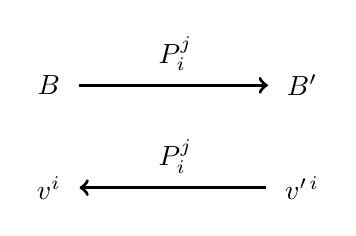
\begin{tikzpicture}
\def\largeur{3.1} \def\hauteur{1.3} \def\decalage{0.4}
\node (A) at (0,\hauteur) {$\mr{B}\ $};
\node (B) at (\largeur,\hauteur) {$\ \mr{B'}$};
\node (C) at (0,0) {$v^i\ $};
\node (D) at (\largeur,0) {$\ v'^{\,i}$};
\node (E) at (0.5*\largeur ,\decalage) {$P_i^j$};
\node (F) at (0.5*\largeur ,\decalage + \hauteur) {$P_i^j$};
\draw[very thick,->] (A)--(B); \draw[very thick,->] (D)--(C);
\end{tikzpicture}
%\end{center}
\end{minipage}
C'est pour cela qu'on appelle contravariante les composantes des vecteurs, elles varient à l'inverse des vecteurs de la base.
\[
[P^{\,i}_j]^{-1} \neq [P^{\,j}_i] \qquad et \qquad V = P V'\ \to\ V'=P'V
\]

\subsection{Fonctions linéaires}
Une application f : (V, $+$,$\cdot$) $\to$ (W, $+$,$\cdot$) est linéaire si :
\[
\forall (\mv{w}, \mv{v})
\]
\subsection{Espace vectoriel dual, V*}

\subsection{Base duale d'une base donnée}


